



\begin{center}
  \begin{figure}[htb]  
   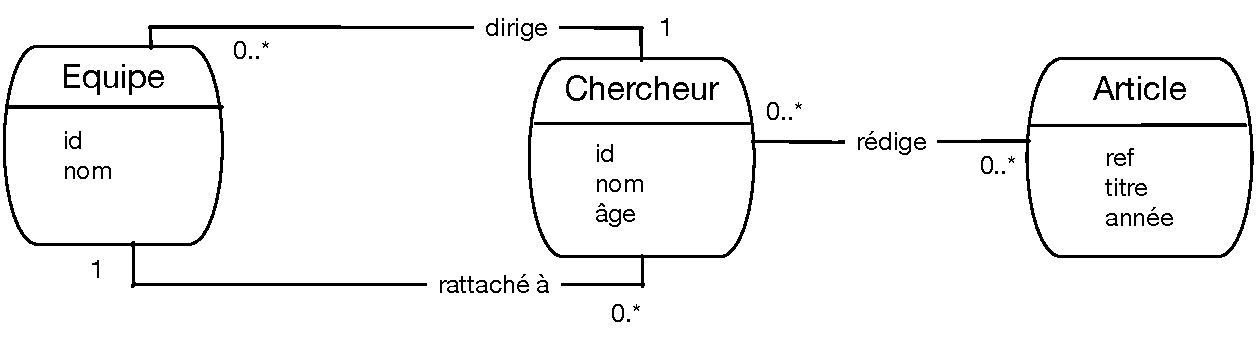
\includegraphics[scale=0.6]{../supports/figures/exam-19-labo}
    \caption{Un laboratoire d'informatique}  
    \label{labo}  
  \end{figure}  
\end{center}

On cherche à modéliser un laboratoire d'informatique afin de pouvoir gérer 
ses équipes, ses chercheurs et leurs publications (articles).
L'analyse donne le schéma  entité/association de la figure~\ref{labo}. 
À partir de cette analyse, quelqu'un propose le schéma 
 relationnel suivant, dans lequel les clés primaires sont en gras
(à vous de trouver les clés étrangères)\,:

\begin{itemize}
  \item {\tt Equipe (\textbf{id}, nom, idDirecteur)}
  \item {\tt Chercheur (\textbf{id}, nom, âge, idEquipe)}
  \item {\tt Article (\textbf{réf}, titre, année)}
  \item {\tt Rédige (\textbf{idChercheur}, réfArticle)} 
\end{itemize}

\section{Conception (6 points)}

\begin{enumerate}
   \item Ce schéma relationnel représente-t-il correctement le modèle conceptuel de la figure~\ref{labo}\,? 
       Vérifiez les clés primaires et étrangères et proposez éventuellement des corrections.

    \item On veut ajouter la position d'un chercheur dans l'ordre des auteurs pour un article. Où
        ajouter cette information, dans le modèle entité association et dans le modèle relationnel\,?
        
    
    \item Un article peut-il être rédigé par des chercheurs
        appartenant à des équipes différentes (justifiez)\,?
    
       \item Un chercheur peut-il diriger une équipe à laquelle
           il n'est pas rattaché (justifiez)\,?

   \item  Donnez les commandes {\tt CREATE TABLE} pour les tables \texttt{Chercheur}, \texttt{Article} et \texttt{Rédige}
       (en tenant compte des corrections éventuelles de la question 1).
\end{enumerate}
    
\begin{solution}


\begin{enumerate}
  \item La clé de {\tt Rédige} doit comprendre {\tt réfArticle}
     en plus de {\tt idAuteur}
   \item On ajoute la position dans l'association \texttt{Rédige} (et dans la table correspondante).
   \item Oui, pas de restriction dans le schéma
   \item Oui, pas de restriction dans le schéma
 \item 
Standard. Exemple pour la relation {\tt Rédige}\,:
\begin{minted}{sql}
CREATE TABLE Redige (idAuteur    int,
                     réfArticle  VARCHAR (10),
                     PRIMARY KEY (idAuteur, réfArticle),
                     FOREIGN KEY (idAuteur) REFERENCES Chercheur,
                     FOREIGN KEY (réfArticle) REFERENCES Article);
\end{minted}


\end{enumerate}

\end{solution}

\section{SQL (8 points)}

Exprimez les requêtes suivantes en SQL.

\begin{enumerate}

\item Noms des chercheurs de l'équipe nommée ``Vertigo''
 \item Titre des articles parus depuis 2015 dont l'un au moins des auteurs appartient à l'équipe ``ROC''
\item Quels articles n'ont pas d'auteur\,?
 \item  Titre des articles parus depuis 2015 dont tous les auteurs appartiennent à l'équipe ``ROC'' (aide\,: 
     la quantification universelle se remplace par la quantification existentielle et la négation)
 \item Nom des chercheurs qui dirigent une équipe à laquelle ils n'appartiennent pas
 \item Nom des chercheurs qui dirigent plus d'une équipe.

\end{enumerate}

\begin{solution}
\begin{minted}{sql}
select e.nom 
from Chercheur as c, Equipe as e
where  e.nom='Vertigo' and c.idEquipe=e.id
\end{minted}

\begin{minted}{sql}
select a.titre 
from Article as a
where  no exists (select 'x' from Rédige where réfArticle=a.réf)
\end{minted}


\begin{minted}{sql}
Select titre
From article a, chercheur c, equipe e, redige r
Where a.ref = r.efarticle
And r.idchercheur=c.id
And c.idequipe=e.id
And a.annee > 2015
And e.nom = 'ROC '
\end{minted}

\begin{minted}{sql}
select nom
from chercheur c, equipe z
where e.idDirecteur=c.id
group by nom
having count(*) >1
\end{minted}

\end{solution}
\section{Algèbre (3 points)}



\begin{enumerate}
   \item Donnez l'expression algébrique pour les deux premières requêtes SQL (section précédente)

   \item Donnez la requête SQL correspondant à l'expression algébrique suivante et expliquez-en le sens.

       $$\pi_{id} (Chercheur) - \pi_{idChercheur} (R\acute{e}dige)$$

\end{enumerate}


\begin{solution}
$\pi_{nom}(\pi_{id} (\sigma_{nom = 'Vertigo'} (Equipe)) \underset{id=idEquipe}{\bowtie} Chercheur )$

Les chercheurs qui n'ont rien publié.


\begin{minted}{sql}
select id
from Chercheur 
where id not in (select idChercheur from Rédige)
\end{minted}


\end{solution}


  
\section{Valeurs nulles ({\bf 2 pts})}

La figure~\ref{ex-relation} montre une instance de {\tt Article}. Les cellules
blanches indiquent des valeurs inconnues.

Donnez le résultat des
requêtes suivantes\,:

\begin{small}
\begin{minted}{sql}
SELECT réf FROM Article WHERE année > 2015
\end{minted}

\begin{minted}{sql}
SELECT réf FROM Article WHERE année <= 2015
\end{minted}

\begin{minted}{sql}
SELECT réf FROM Article WHERE annee > 0 OR titre IS NOT NULL
\end{minted}



\begin{minted}{sql}
SELECT réf FROM Article WHERE (année < 2015 OR année IS NULL) AND titre LIKE `%`
\end{minted}
\end{small}

\begin{figure}[ht]
\begin{center}
\begin{tabular}{c|c|c}
réf  & titre & année \\\hline
AR243 & Les ordinateurs pensent-ils? & 2018  \\\hline 
AR254 & Money for nothing &  \\\hline
AR20 &  & 2010\\\hline
\end{tabular}
\end{center}
\caption{Une instance de la relation {\tt Article}}
\label{ex-relation}
\end{figure}


\begin{solution}
   \begin{enumerate}
      \item AR243
       \item AR20
       \item AR243, AR254, AR20
         \item AR254
    \end{enumerate}
\end{solution}


\section{Transactions ({\bf 1 pt})}

Soit deux transactions concurrentes  $T_1$ et  $T_2$. Quelle(s) affirmation(s), parmi les suivantes, est (sont) vraie(s) 
dans un système transactionnel assurant les propriétés ACID
en isolation complète.

\begin{enumerate}
   \item  Si $T_2$  débute après $T_1$,
       $T_1$  ne voit jamais les  mises à jour de $T_2$.
   
   \item $T_1$  ne voit pas ses propres mises à jour tant qu'elle n'a pas validé.
   
  \item Si $T_2$  débute après $T_1$,
       $T_1$  ne voit les  mises à jour de $T_2$ qu'après  que $T_2$ a effectué un \texttt{commit}.

  \item Si  $T_1$  et $T_2$  veulent modifier le même nuplet,
       cela déclenche un interblocage (\texttt{deadlock}).
   
\end{enumerate}


\begin{solution}
Seule la première affirmation est vraie
\end{solution}
